\documentclass[12pt]{jarticle}
\usepackage{a4wide}
\usepackage{amsmath}%数学記号
\usepackage{amssymb}%数学記号
\usepackage{epsfig}%図
\usepackage{latexsym}
\usepackage{supertabular}
\usepackage{graphicx}
\usepackage{color}
\usepackage{ascmac}
\usepackage{multicol}
\usepackage{ascmac}
\usepackage{systeme}
\usepackage{amsmath,cases}
\usepackage{float}
\usepackage{here}
\usepackage{otf}
\pagestyle{plain}

\newtheorem{theorem}{定理}[section]
\newtheorem{lemma}[theorem]{補題}
\newtheorem{proposition}[theorem]{命題}
\newtheorem{conjecture}[theorem]{予想}
\newtheorem{corollary}[theorem]{系}
\newtheorem{definition}[theorem]{定義}
\newtheorem{example}[theorem]{例}
\newtheorem{exercise}[theorem]{例題}
\newtheorem{problem}[theorem]{問}
\newtheorem{algorithm}[theorem]{アルゴリズム}
\newtheorem{remark}[theorem]{注意}

\def\qed{{\hfill$\square$}}
\def\proof{{\vspace{-0.3cm}f 証明: \,}}
\def\solution{{\vspace{-0.3cm}f 解: \,}}
\def\N{{\Bbb N}}
\def\Z{{\Bbb Z}}
\def\Q{{\Bbb Q}}
\def\R{{\Bbb R}}
\def\C{{\Bbb C}}
\def\F{{\Bbb F}}
\def\D{{\mathcal D}}
\def\mod{{\mathrm{mod\,\,}}}
\def\GL{{\mathrm{GL}}}
\def\GF{{\mathrm{GF}}}
\def\H{{\mathcal{H}}}

\setlength{\textwidth}{170mm}
\setlength{\textheight}{240mm}
\setlength{\oddsidemargin}{-5mm}
\setlength{\evensidemargin}{-5mm}
\setlength{\topmargin}{-10mm}
\setlength{\headheight}{0mm}
\setlength{\headsep}{10mm}

\title{項目反応理論}
\begin{document}
\maketitle
\section{項目反応理論による評価を加味した数学テストとe-learningシステムへの実装の試み}
前回は教職教養の問題を題材に項目特性図を用いて、テスト分析を行った。その最後で数学のテストへの適用に関心を示した。そこで今回は、九州工業大学の広瀬英雄教授や月原由紀、鈴木敬一らの論文をもとに、実際に数学のテストで応用した例を紹介する。%して、自分で組んだプログラムを紹介できれば良いな
\subsection{はじめに}
項目反応理論は、英語能力判定としてTOEFLやTOEICテストに使われ定着している。大学数学などでは、正解不正解といった$2$値応答の問題を作りにくいこともあってか、IRTを積極的に用いてテスト分析に応用した実例は少ない。
\subsection{IRT(Item Response Theory)とは}
従来の古典的テスト評価法は、単に問題に配点を与えておき、各問題における得点を合計したもので総合評価が与えられるので、個々の問題の特性や受験者の能力などは加味されてないといえる。IRTは問題の特性と学生の能力を同時に取り扱うことができる総合的な評価になっている。従って、古典的評価法では同点であっても、難問に解答した割合が多いほど評価値は高くなる傾向がある。
\subsubsection{IRTによるもでるについて}
今回は$2$母数ロジスティックモデルを用いて考える。学生$i$が能力$\theta_i$を持ち、テストの$j$番目の項目に正解できる確率$P_j(\theta_i)$を
\begin{align}
  \label{00}
  \displaystyle P_j(\theta_i) = \frac{1}{1 + \exp{-1.7a_j}(\theta_i - b_j)} \tag{1}
\end{align}
と表すことができた。ここで$a_j$は問題の識別力、$b_j$は問題の困難度とする。この$P_j(\theta_i)$を縦軸に、横軸を能力$\theta$としたグラフをICC(項目特性曲線)と呼ぶ。
\newpage
\begin{figure}[H]
  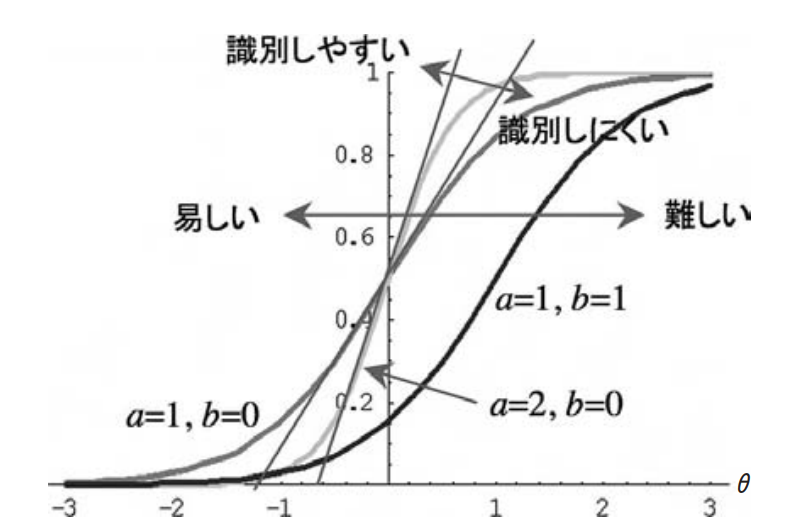
\includegraphics[bb = -300 300 1 1,scale = 0.4]{01.png}
  \vspace{4cm}
  \caption{ICCの見方}
\end{figure}
\subsection{IRT評価と素点評価の比較}
テストは被験者が紙に答案を書く一般的な形式で行われている。次の表はある学科での正答、誤答の反応パタンでありグラフは推定された項目特性曲線である。
\begin{figure}[H]
  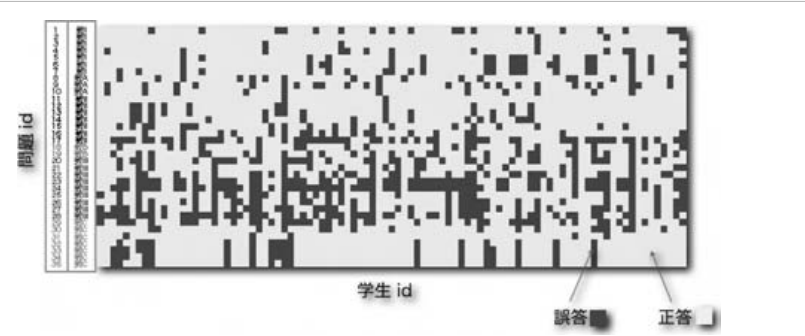
\includegraphics[bb = -230 300 1 1,scale = 0.5]{02.png}
  \vspace{4.5cm}
  \caption{反応パタン}
\end{figure}
\begin{figure}[H]
  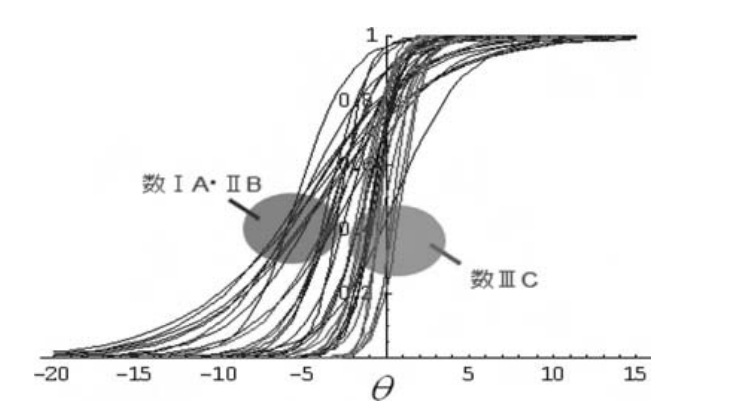
\includegraphics[bb = -230 300 1 1,scale = 0.5]{03.png}
  \vspace{4.8cm}
  \caption{ICC}
\end{figure}
図$3$、図$4$より数IIIの難易度は高く、問題の識別力も高いことが示されいている。
また、以下の図により、同じの素点をとっても能力値に幅が観測されることがわかる。
\begin{figure}[H]
  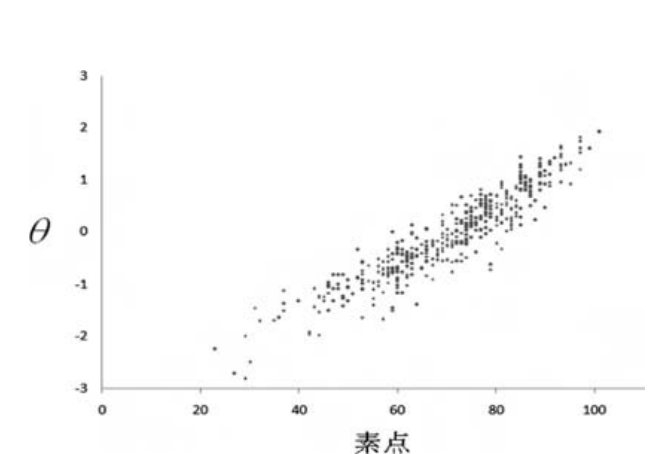
\includegraphics[bb = -200 300 1 1,scale = 0.5]{04.png}
  \vspace{4.8cm}
  \caption{ICC}
\end{figure}
例えば、素点$60$点では、$\theta$は$0$から$-1.5$までばらついている。逆に$\theta = 0$でも素点は$60$点から$80$点までばらついている。このことから、能力と点数が逆転することも考えられる。$1$回だけのテストでは決定的な判断をするのが難しくなる。誤差が確率的にどのくらいの割合で観察されるのかを検証しておく必要がある。
\end{document}
